\documentclass[10pt,aspectratio=169]{beamer}
\usetheme{Boadilla}
\usecolortheme{dove}

\usepackage{amsmath}
\usepackage{booktabs}
\usepackage{graphicx}
\usepackage{array}
\usepackage{listings}
\usepackage{tikz}
\usepackage{url}
\usetikzlibrary{arrows.meta,positioning}

\graphicspath{{../figures/}}
\providecommand{\YearEarlyOne}{1945}
\providecommand{\CapacityGrowthEarlyOne}{1.286}
\providecommand{\CapitalGrowthEarlyOne}{0.692}
\providecommand{\RatioEarlyOne}{1.86}
\providecommand{\YearEarlyTwo}{1946}
\providecommand{\CapacityGrowthEarlyTwo}{4.691}
\providecommand{\CapitalGrowthEarlyTwo}{9.572}
\providecommand{\RatioEarlyTwo}{0.49}
\providecommand{\OrthTheta}{0.23784}
\providecommand{\PrimitiveTheta}{0.34143}
\providecommand{\OrthPsi}{0.31207}
\providecommand{\PrimitivePsi}{0.27696}
\providecommand{\InteractionLambda}{-1.02937}
\providecommand{\OrthPrimitiveFitDifference}{4.8e-14}
\providecommand{\SthirtyFourResidualDifference}{6.8e-16}
\providecommand{\CompositionShare}{58.0}
\providecommand{\CompositionShareLow}{49.8}
\providecommand{\CompositionShareHigh}{67.6}
\providecommand{\DenominatorShare}{26.2}
\providecommand{\DistributionShare}{1.2}
\providecommand{\ScaleReferenceShare}{14.6}
\providecommand{\TopTwoInfluenceShare}{54.7}
\providecommand{\FirstYearDropReduction}{52.5}
\providecommand{\CapacityGrowthRoughness}{0.0001008}
\providecommand{\RatioRoughness}{0.1236}
\providecommand{\ConstantDenominatorRoughness}{0.04053}
\providecommand{\RhoNfcGva}{0.98}
\providecommand{\RhoNfcGvaLow}{0.92}
\providecommand{\RhoNfcGvaHigh}{0.98}
\providecommand{\HalfLifeNfcGva}{34.3}
\providecommand{\RhoNfcNva}{0.96}
\providecommand{\RhoNfcNvaLow}{0.77}
\providecommand{\RhoNfcNvaHigh}{0.98}
\providecommand{\HalfLifeNfcNva}{17.0}
\providecommand{\MtwoLambdaGvaHthree}{-28.00}
\providecommand{\MtwoLambdaGvaHfive}{-27.31}
\providecommand{\MtwoLambdaNvaHthree}{-12.76}
\providecommand{\MtwoLambdaNvaHfive}{-3.85}
\providecommand{\MthreeLambdaGva}{60.54}
\providecommand{\MthreeLambdaNva}{-12.43}
\providecommand{\BootstrapReplications}{1000}
\providecommand{\ValidationCheckCount}{8}
\providecommand{\ClaimCheckCount}{36}
\providecommand{\AnchorYear}{1973}
\providecommand{\CoefficientTolerance}{5\times10^{-5}}
\providecommand{\AlgebraTolerance}{10^{-10}}
\providecommand{\LineSthirtyFourOrth}{370}
\providecommand{\LineSthirtyFiveFmols}{127}
\providecommand{\LineReconstructionRatio}{128}
\providecommand{\LineSninetyBacktransform}{449}
\providecommand{\HashSthirtyFour}{afce5b84b7}
\providecommand{\HashSthirtyFive}{727e736cea}
\providecommand{\HashReconstruction}{a263c1caef}
\providecommand{\HashSninety}{2899921142}


\setbeamertemplate{navigation symbols}{}
\setbeamertemplate{headline}{}
\setbeamercolor{titlelike}{parent=structure,bg=gray!10}
\setbeamercolor{item}{fg=gray!80}
\setbeamercolor{block title}{bg=gray!20,fg=black}
\setbeamercolor{block body}{bg=gray!5,fg=black}
\setbeamercolor{alertblock title}{bg=red!16,fg=black}
\setbeamercolor{alertblock body}{bg=red!4,fg=black}
\setlength{\parskip}{0pt}
\setbeamertemplate{itemize/enumerate body begin}{\vspace{-0.15em}}
\setbeamertemplate{itemize/enumerate subbody begin}{\vspace{-0.15em}}

\definecolor{pathred}{HTML}{B2182B}
\definecolor{pathblue}{HTML}{2166AC}
\definecolor{pathgreen}{HTML}{4D9221}
\definecolor{pathpurple}{HTML}{762A83}

\lstset{
  basicstyle=\ttfamily\fontsize{6.2}{7.1}\selectfont,
  breaklines=true,
  columns=fullflexible,
  frame=single,
  rulecolor=\color{gray!35},
  backgroundcolor=\color{gray!4},
  showstringspaces=false
}

\title[Why the red path is lumpy]{Why the Red Capacity-Payoff Path Is Lumpy}
\subtitle{Economic interpretation and source-to-result audit}
\author{Dissertation Chapter 2}
\date{July 2026}

\newcommand{\sourcefooter}[1]{%
  \par\vfill{\tiny\color{gray!70}Evidence source: #1}\vspace{-0.35em}}

\setbeamertemplate{footline}{%
  \leavevmode%
  \hbox{%
  \begin{beamercolorbox}[wd=.82\paperwidth,ht=2.4ex,dp=1.1ex,leftskip=1em]{author in head/foot}%
    \insertshorttitle\hfill Script-grounded S90 diagnostic
  \end{beamercolorbox}%
  \begin{beamercolorbox}[wd=.18\paperwidth,ht=2.4ex,dp=1.1ex,center]{date in head/foot}%
    \insertframenumber/\inserttotalframenumber
  \end{beamercolorbox}}%
}

\begin{document}

% Main 1
\begin{frame}{The instability appears after estimation, during reconstruction}
  \begin{columns}[T,onlytextwidth]
    \begin{column}{0.62\textwidth}
      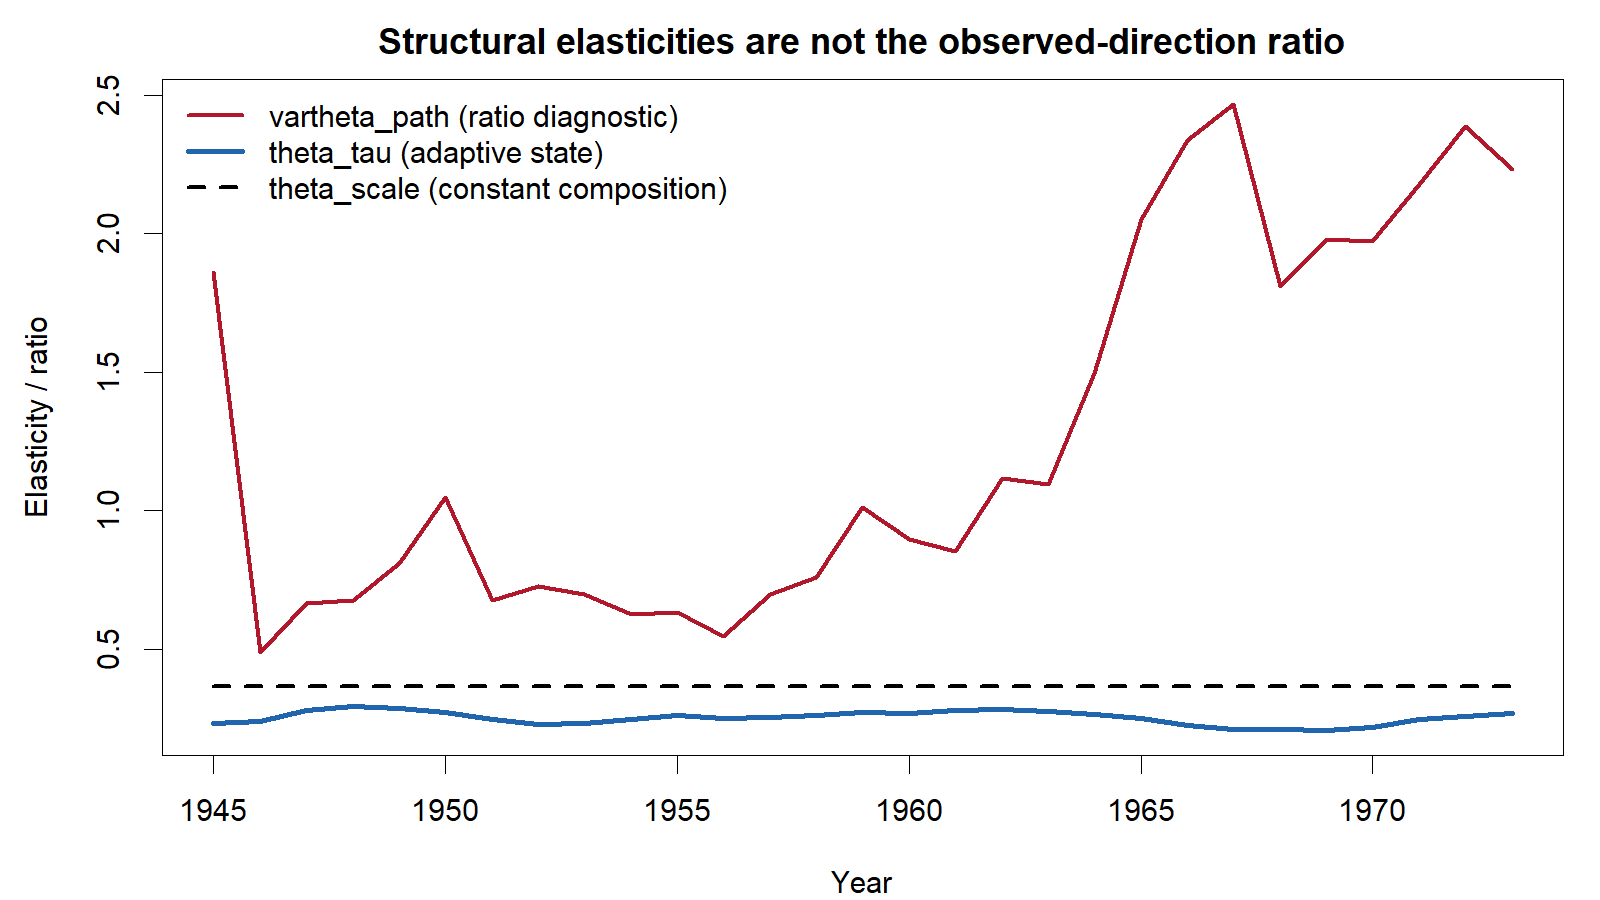
\includegraphics[width=\linewidth]{F02_structural_vs_directional.png}
    \end{column}
    \begin{column}{0.35\textwidth}
      \begin{alertblock}{The central distinction}
        The red line is not an equilibrium elasticity. It is capacity growth divided by aggregate capital growth in each observed year.
      \end{alertblock}
      \begin{itemize}\small
        \item The scale elasticity is constant within an estimated window.
        \item The technique elasticity moves with a wage-pressure state.
        \item The red ratio also moves with the annual mix and speed of capital accumulation.
      \end{itemize}
    \end{column}
  \end{columns}
  \sourcefooter{\texttt{US\_S90\_path\_dependent\_theta\_robustness.R} and \texttt{S90\_reconstructed\_path\_roughness\_comparison.csv}}
\end{frame}

% Main 2
\begin{frame}{Capacity can expand by enlarging plant or changing technique}
  \begin{columns}[T,onlytextwidth]
    \begin{column}{0.48\textwidth}
      \begin{block}{Scale: more productive space}
        \centering
        \Large $g_t^{NRC}$

        \vspace{0.5em}\normalsize
        Structures measure the extension of plant, buildings, and the physical layout of production.
      \end{block}
      \begin{itemize}\small
        \item Balanced accumulation expands machinery and structures together.
        \item Its capacity payoff is governed by $\theta^{scale}=\theta$.
      \end{itemize}
    \end{column}
    \begin{column}{0.48\textwidth}
      \begin{block}{Composition: more machinery per unit of plant}
        \centering
        \Large $\Delta\tau_t=g_t^{ME}-g_t^{NRC}$

        \vspace{0.5em}\normalsize
        Positive $\Delta\tau_t$ means that the installed technique becomes more machinery-intensive.
      \end{block}
      \begin{itemize}\small
        \item Rapid mechanization changes the direction of accumulation.
        \item Its capacity payoff is governed by $\theta_t^{\tau}$.
      \end{itemize}
    \end{column}
  \end{columns}
  \begin{block}{The growth accounting identity}
    \centering
    \Large $g_t^p=\theta^{scale}g_t^{NRC}+\theta_t^{\tau}(g_t^{ME}-g_t^{NRC})$
  \end{block}
  \sourcefooter{\texttt{US\_S90\_path\_dependent\_theta\_robustness.R}: corrected primitive-basis \texttt{build\_path}}
\end{frame}

% Main 3
\begin{frame}{The three objects answer different economic questions}
  \renewcommand{\arraystretch}{1.35}
  \begin{table}
    \centering
    \small
    \begin{tabular}{@{}p{0.20\textwidth}p{0.47\textwidth}p{0.25\textwidth}@{}}
      \toprule
      \textbf{Object} & \textbf{Question answered} & \textbf{Economic status} \\
      \midrule
      $\theta^{scale}=\theta$ & If structures and machinery expand proportionally, how much does capacity expand? & Equilibrium scale elasticity \\
      $\theta_t^{\tau}=\psi+\lambda\widetilde d_t$ & At the current wage-pressure state, what is the capacity payoff from greater machinery intensity? & State-conditioned technique elasticity \\
      $\vartheta_t^{path}=g_t^p/g_t^{cap}$ & How much capacity growth occurred per unit of measured aggregate capital growth in this particular year? & Realized-direction ratio \\
      \bottomrule
    \end{tabular}
  \end{table}
  \begin{alertblock}{Interpretive rule}
    A volatile $\vartheta_t^{path}$ does not imply a volatile equilibrium frontier. It can move because the economy changes the composition of investment or because $g_t^{cap}$ changes sharply.
  \end{alertblock}
  \sourcefooter{\texttt{reconstruct\_golden\_age\_paths.R} and \texttt{S90\_original\_vartheta\_path\_exact\_contribution\_ledger.csv}}
\end{frame}

% Main 4
\begin{frame}{Higher capacity growth can produce a lower capacity-payoff ratio}
  \begin{columns}[T,onlytextwidth]
    \begin{column}{0.66\textwidth}
      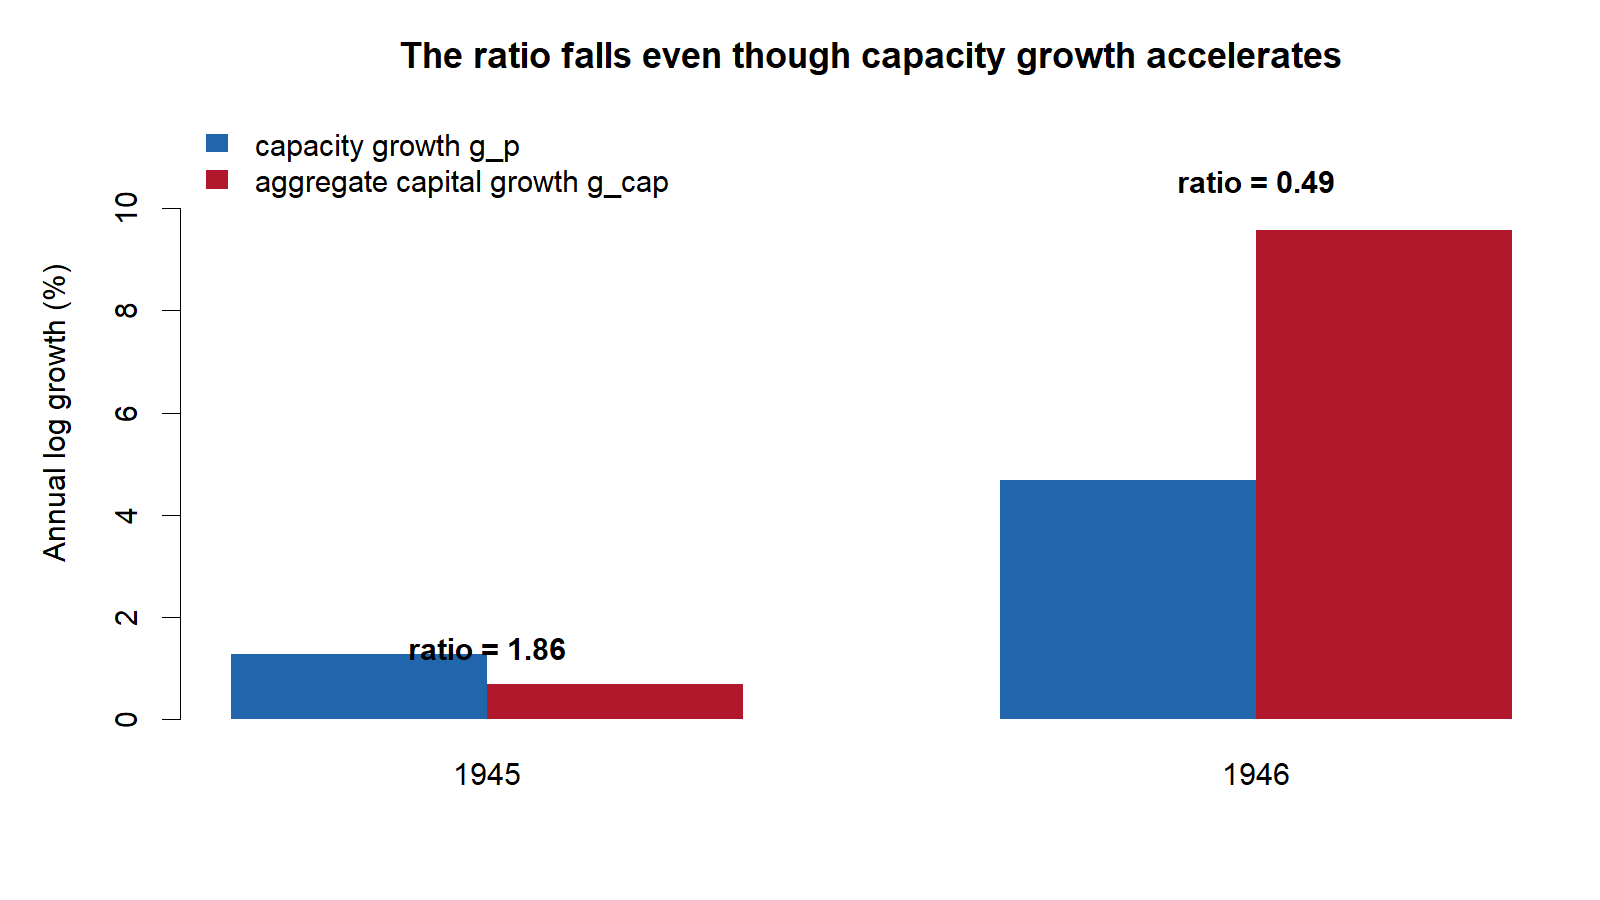
\includegraphics[width=\linewidth]{F07_two_year_ratio_arithmetic.png}
    \end{column}
    \begin{column}{0.31\textwidth}
      \small
      \begin{block}{\YearEarlyOne}
        $g^p=\CapacityGrowthEarlyOne\%$

        $g^{cap}=\CapitalGrowthEarlyOne\%$

        $g^p/g^{cap}=\mathbf{\RatioEarlyOne}$
      \end{block}
      \begin{block}{\YearEarlyTwo}
        $g^p=\CapacityGrowthEarlyTwo\%$

        $g^{cap}=\CapitalGrowthEarlyTwo\%$

        $g^p/g^{cap}=\mathbf{\RatioEarlyTwo}$
      \end{block}
      Capacity grows faster in the second year, but aggregate capital grows faster still. The ratio therefore falls.
    \end{column}
  \end{columns}
  \sourcefooter{D10 capital levels reproduced by \texttt{US\_S90\_beamer\_source\_audit.R}}
\end{frame}

% Main 5
\begin{frame}{The red path has a traceable four-script origin}
  \centering
  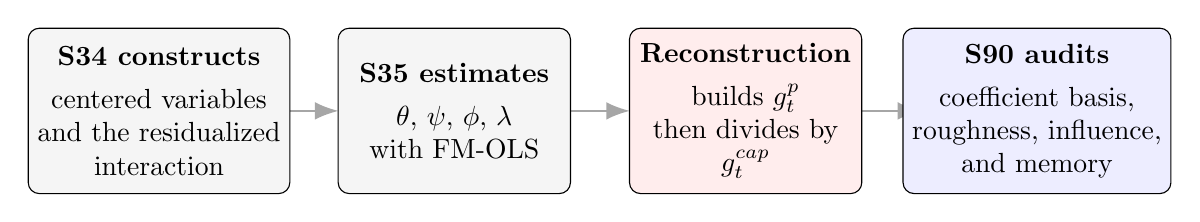
\begin{tikzpicture}[node distance=0.55cm, every node/.style={align=center}]
    \draw[-{Latex[length=3mm]},thick,gray!70] (3.05,0) -- (3.80,0);
    \draw[-{Latex[length=3mm]},thick,gray!70] (6.75,0) -- (7.50,0);
    \draw[-{Latex[length=3mm]},thick,gray!70] (10.45,0) -- (11.20,0);
    \node[draw,rounded corners,fill=gray!8,minimum width=3.05cm,minimum height=2.1cm] at (1.52,0)
      {\textbf{S34 constructs}\\[0.35em] centered variables\\and the residualized\\interaction};
    \node[draw,rounded corners,fill=gray!8,minimum width=2.95cm,minimum height=2.1cm] at (5.27,0)
      {\textbf{S35 estimates}\\[0.35em] $\theta$, $\psi$, $\phi$, $\lambda$\\with FM-OLS};
    \node[draw,rounded corners,fill=red!7,minimum width=2.95cm,minimum height=2.1cm] at (8.97,0)
      {\textbf{Reconstruction}\\[0.35em] builds $g_t^p$\\then divides by\\$g_t^{cap}$};
    \node[draw,rounded corners,fill=blue!7,minimum width=2.95cm,minimum height=2.1cm] at (12.67,0)
      {\textbf{S90 audits}\\[0.35em] coefficient basis,\\roughness, influence,\\and memory};
  \end{tikzpicture}

  \vspace{1em}
  \begin{alertblock}{Where the visual instability enters}
    S34 and S35 estimate a levels relationship. The annual red path is created later, when the reconstruction script converts those coefficients into capacity growth and divides by annual aggregate capital growth.
  \end{alertblock}
  \sourcefooter{Source anchors and hashes: \texttt{S90\_beamer\_script\_provenance\_ledger.csv}}
\end{frame}

% Main 6
\begin{frame}{Orthogonalization relabels coefficients but leaves fitted capacity unchanged}
  \begin{columns}[T,onlytextwidth]
    \begin{column}{0.55\textwidth}
      \begin{block}{Residual-centered interaction}
        \small
        \[
        r_t=(\widetilde\tau_t\widetilde d_t)
        -\delta_0-\delta_k\widetilde k_t^{NRC}
        -\delta_{\tau}\widetilde\tau_t-\delta_d\widetilde d_t.
        \]
        The residual is orthogonal to the linear regressors, which improves numerical conditioning.
      \end{block}
      \begin{alertblock}{The economic derivative still requires the primitive basis}
        \[
        \psi^{primitive}=\psi^{orth}-\lambda\delta_{\tau},\qquad
        \theta^{primitive}=\theta^{orth}-\lambda\delta_k.
        \]
      \end{alertblock}
    \end{column}
    \begin{column}{0.41\textwidth}
      \small
      \begin{tabular}{@{}lrr@{}}
        \toprule
        & \textbf{orthogonal} & \textbf{primitive} \\
        \midrule
        $\theta$ & \OrthTheta & \PrimitiveTheta \\
        $\psi$   & \OrthPsi   & \PrimitivePsi \\
        $\lambda$ & \InteractionLambda & \InteractionLambda \\
        \bottomrule
      \end{tabular}

      \vspace{1em}
      \begin{block}{Audit result}
        Fitted values agree to \texttt{\OrthPrimitiveFitDifference}. The back-transformation changes coefficient interpretation, not the fitted capacity schedule.
      \end{block}
    \end{column}
  \end{columns}
  \sourcefooter{S34 full-panel residualization and S35 Golden-Age coefficients, independently reproduced in the Beamer claim ledger}
\end{frame}

% Main 7
\begin{frame}{The reconstruction script converts smooth effects into an annual flow ratio}
  \begin{columns}[T,onlytextwidth]
    \begin{column}{0.22\textwidth}
      \begin{block}{Estimated inputs}
        \centering
        $\theta,\ \psi,\ \lambda$
      \end{block}
    \end{column}
    \begin{column}{0.03\textwidth}\centering $\rightarrow$\end{column}
    \begin{column}{0.27\textwidth}
      \begin{block}{Technique payoff}
        \centering
        $\theta_t^{ME}=\psi+\lambda\widetilde\omega_t$

        $\theta_t^{NRC}=\theta-\theta_t^{ME}$
      \end{block}
    \end{column}
    \begin{column}{0.03\textwidth}\centering $\rightarrow$\end{column}
    \begin{column}{0.22\textwidth}
      \begin{block}{Capacity growth}
        \centering
        $g_t^p=\theta_t^{NRC}g_t^{NRC}+\theta_t^{ME}g_t^{ME}$
      \end{block}
    \end{column}
    \begin{column}{0.03\textwidth}\centering $\rightarrow$\end{column}
    \begin{column}{0.17\textwidth}
      \begin{alertblock}{Red path}
        \centering
        $\displaystyle\frac{g_t^p}{g_t^{cap}}$
      \end{alertblock}
    \end{column}
  \end{columns}

  \vspace{1em}
  \begin{block}{The label created the confusion}
    The script saves the final ratio as \texttt{theta\_total\_t}. That variable name suggests a structural elasticity even though the expression is an annual realized-capacity payoff.
  \end{block}
  \sourcefooter{\texttt{reconstruct\_golden\_age\_paths.R}, source line \LineReconstructionRatio; reconstruction series reproduced to numerical precision}
\end{frame}

% Main 8
\begin{frame}{Capacity growth is far smoother than the ratio formed from it}
  \begin{columns}[T,onlytextwidth]
    \begin{column}{0.72\textwidth}
      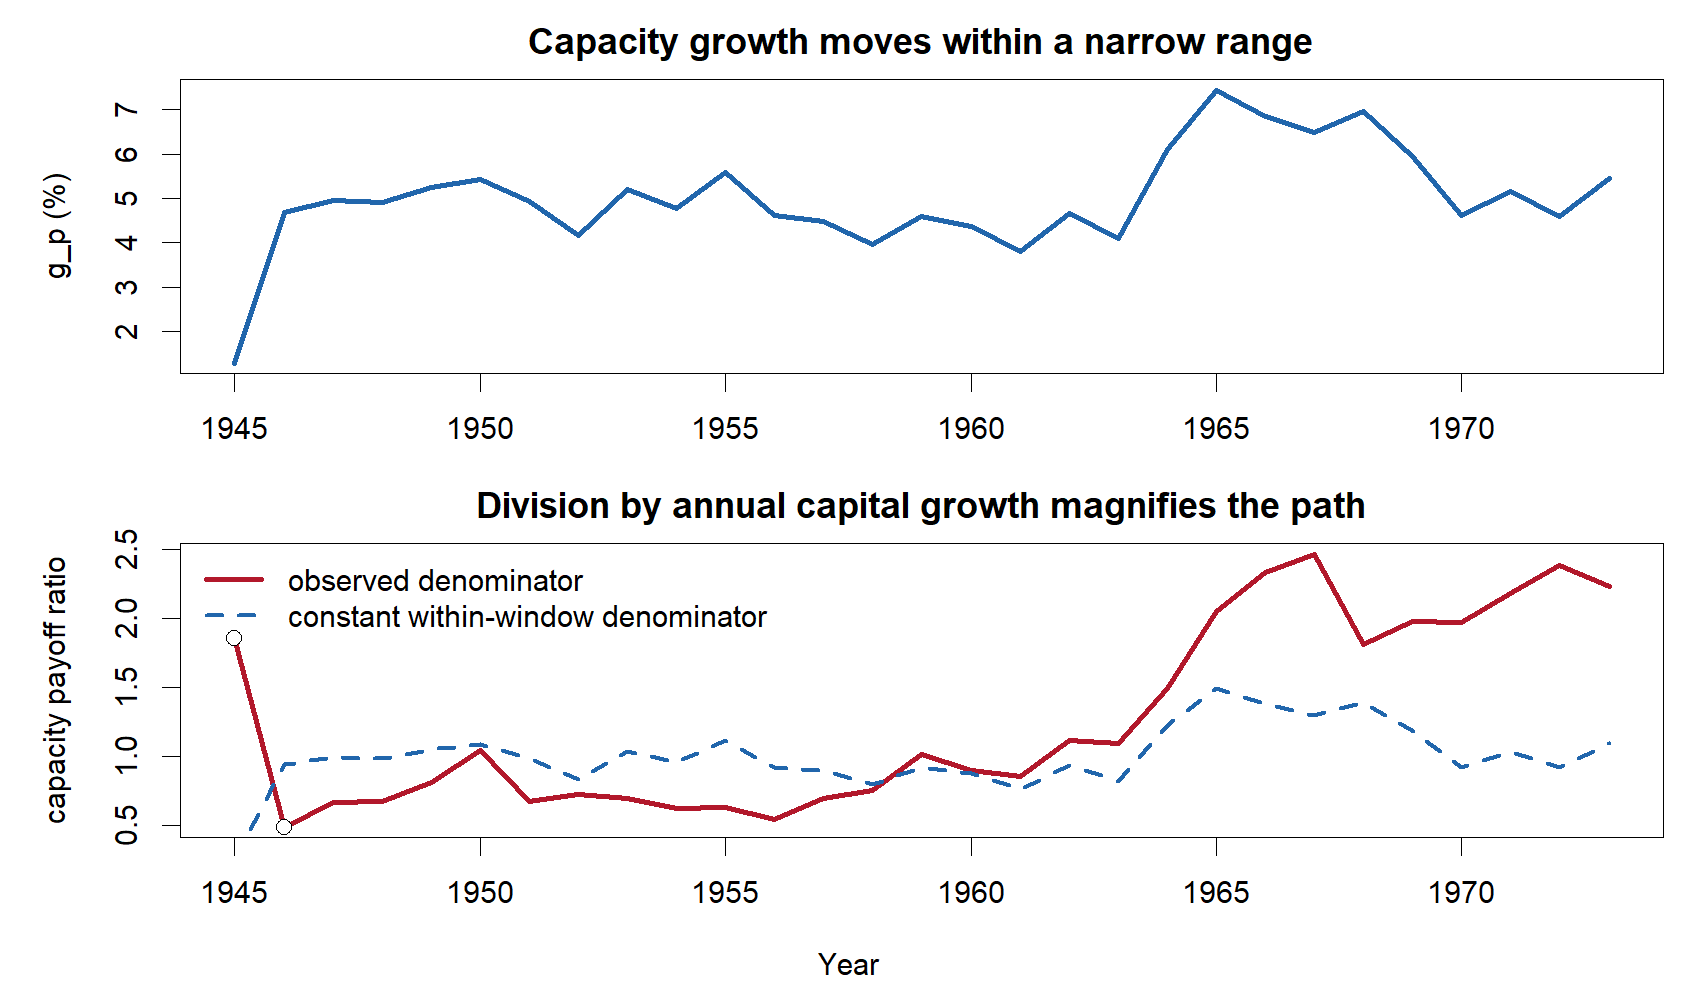
\includegraphics[width=\linewidth]{F08_capacity_growth_and_denominator_amplification.png}
    \end{column}
    \begin{column}{0.25\textwidth}
      \small
      \begin{block}{First-difference roughness}
        \begin{tabular}{@{}lr@{}}
          $g_t^p$ & \CapacityGrowthRoughness \\
          red ratio & \RatioRoughness \\
          fixed $\bar g^{cap}$ & \ConstantDenominatorRoughness \\
        \end{tabular}
      \end{block}
      \begin{alertblock}{Meaning}
        The denominator magnifies the path, but the fixed-denominator line still moves. Composition therefore remains part of the explanation.
      \end{alertblock}
    \end{column}
  \end{columns}
  \sourcefooter{\texttt{S90\_denominator\_amplification\_ledger.csv} and independently reconstructed D10 growth rates}
\end{frame}

% Main 9
\begin{frame}{The exact decomposition isolates the economic channels}
  \vspace{-0.35em}
  \begin{block}{Exact identity}
    \centering
    $\displaystyle
    \vartheta_t^{path}
    =\frac{\theta g_t^{NRC}}{g_t^{cap}}
    +\frac{\psi(g_t^{ME}-g_t^{NRC})}{g_t^{cap}}
    +\frac{\lambda\widetilde d_t(g_t^{ME}-g_t^{NRC})}{g_t^{cap}}.$
  \end{block}
  \vspace{-0.5em}
  \centering
  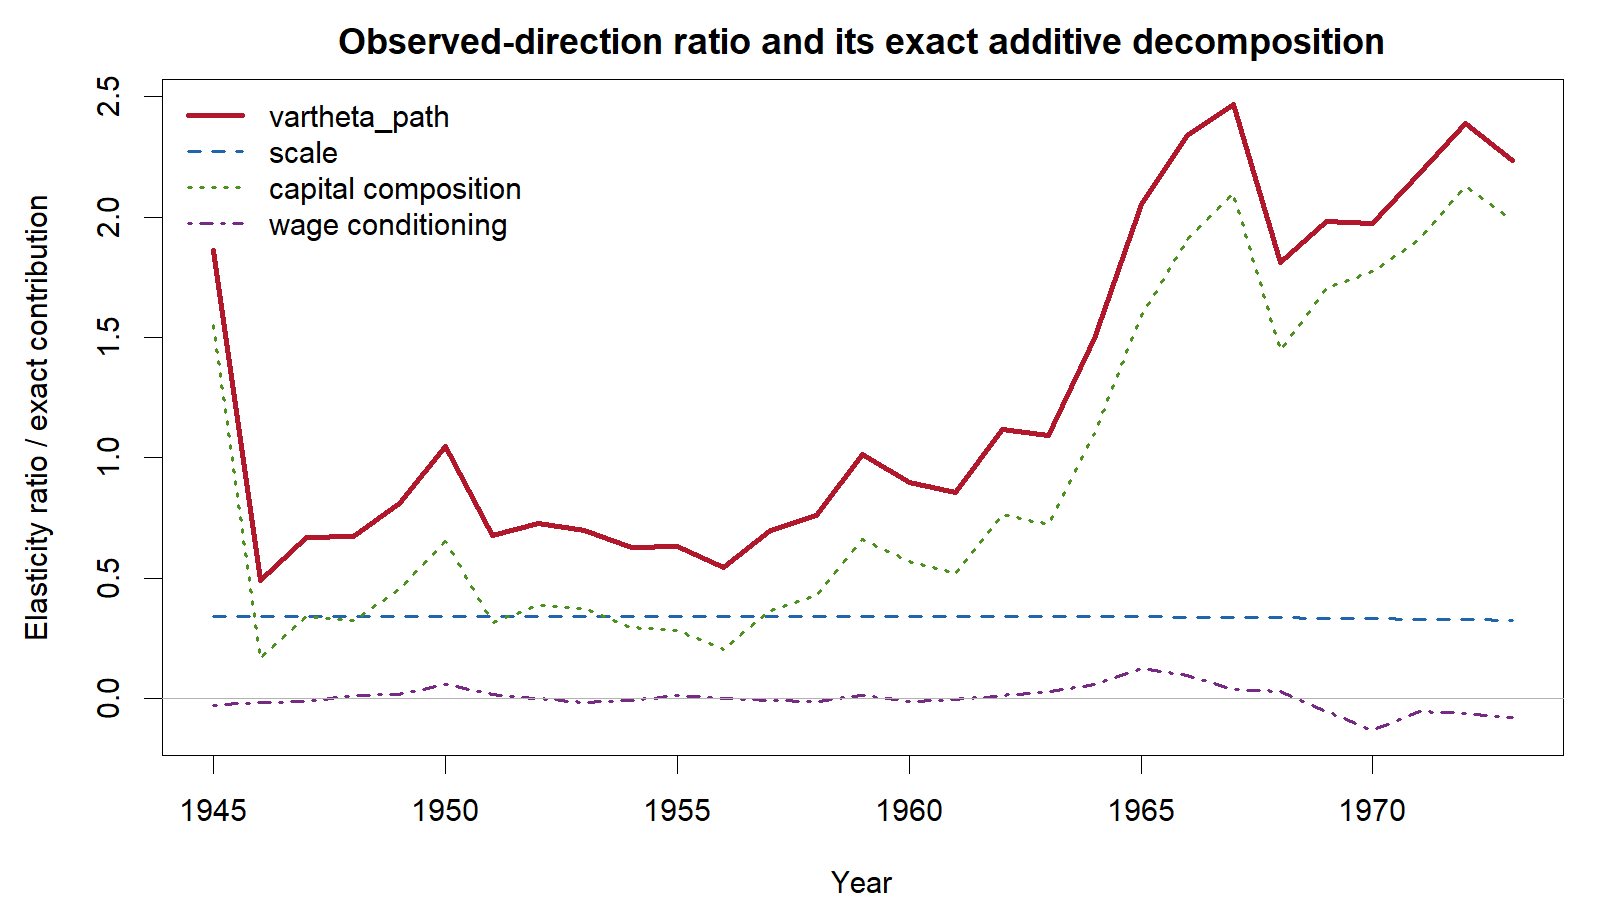
\includegraphics[width=0.55\linewidth]{F01_original_lumpiness_decomposition.png}
  \vspace{-0.4em}

  \small The wage-conditioned contribution remains close to zero. The visible rise and fall follows the accumulation-composition term.
  \sourcefooter{\texttt{S90\_original\_vartheta\_path\_exact\_contribution\_ledger.csv}; maximum identity error below numerical tolerance}
\end{frame}

% Main 10
\begin{frame}{Composition is point-dominant, but the evidence is not decisive}
  \begin{columns}[T,onlytextwidth]
    \begin{column}{0.69\textwidth}
      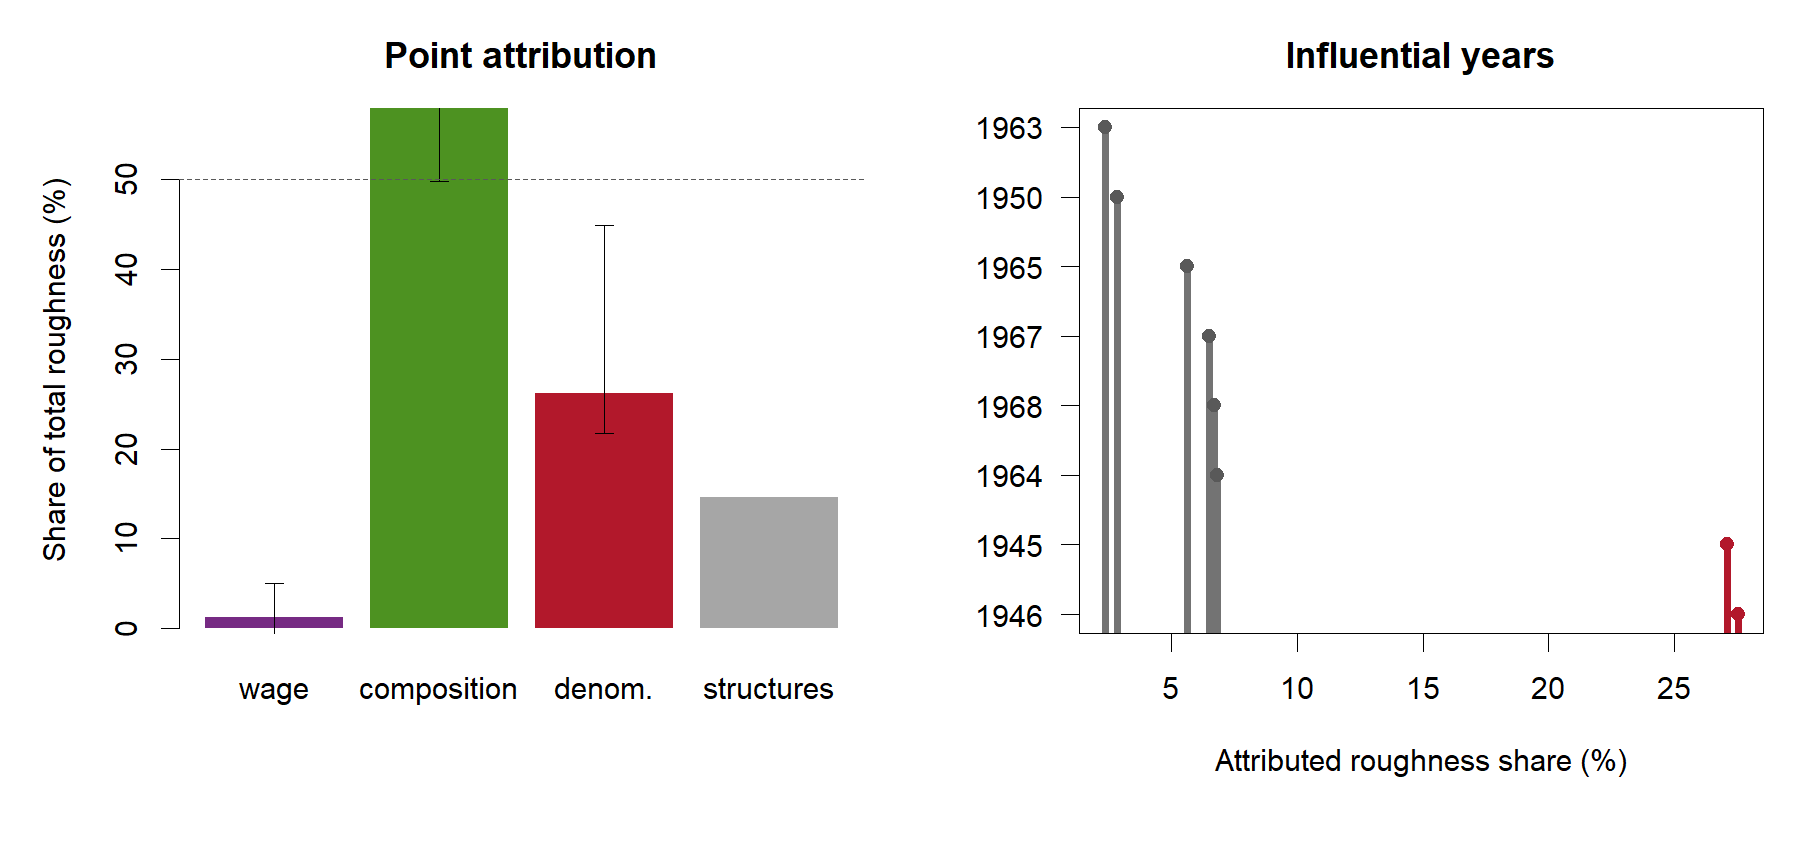
\includegraphics[width=\linewidth]{F09_roughness_attribution_and_influence.png}
    \end{column}
    \begin{column}{0.28\textwidth}
      \small
      \begin{itemize}
        \item Composition: \textbf{\CompositionShare\%}
        \item Denominator: \DenominatorShare\%
        \item Wage conditioning: \DistributionShare\%
        \item Structures reference: \ScaleReferenceShare\%
      \end{itemize}
      \begin{alertblock}{Two qualifications}
        The composition interval is \CompositionShareLow-\CompositionShareHigh\%, crossing the majority threshold.

        The \YearEarlyOne-\YearEarlyTwo observations account for \TopTwoInfluenceShare\% of attributed roughness.
      \end{alertblock}
    \end{column}
  \end{columns}
  \sourcefooter{\texttt{S90\_shapley\_roughness\_attribution\_ledger.csv} and \texttt{S90\_capital\_growth\_and\_influential\_year\_audit.csv}}
\end{frame}

% Main 11
\begin{frame}{Path dependence attaches wage history to newly installed technique}
  \begin{columns}[T,onlytextwidth]
    \begin{column}{0.58\textwidth}
      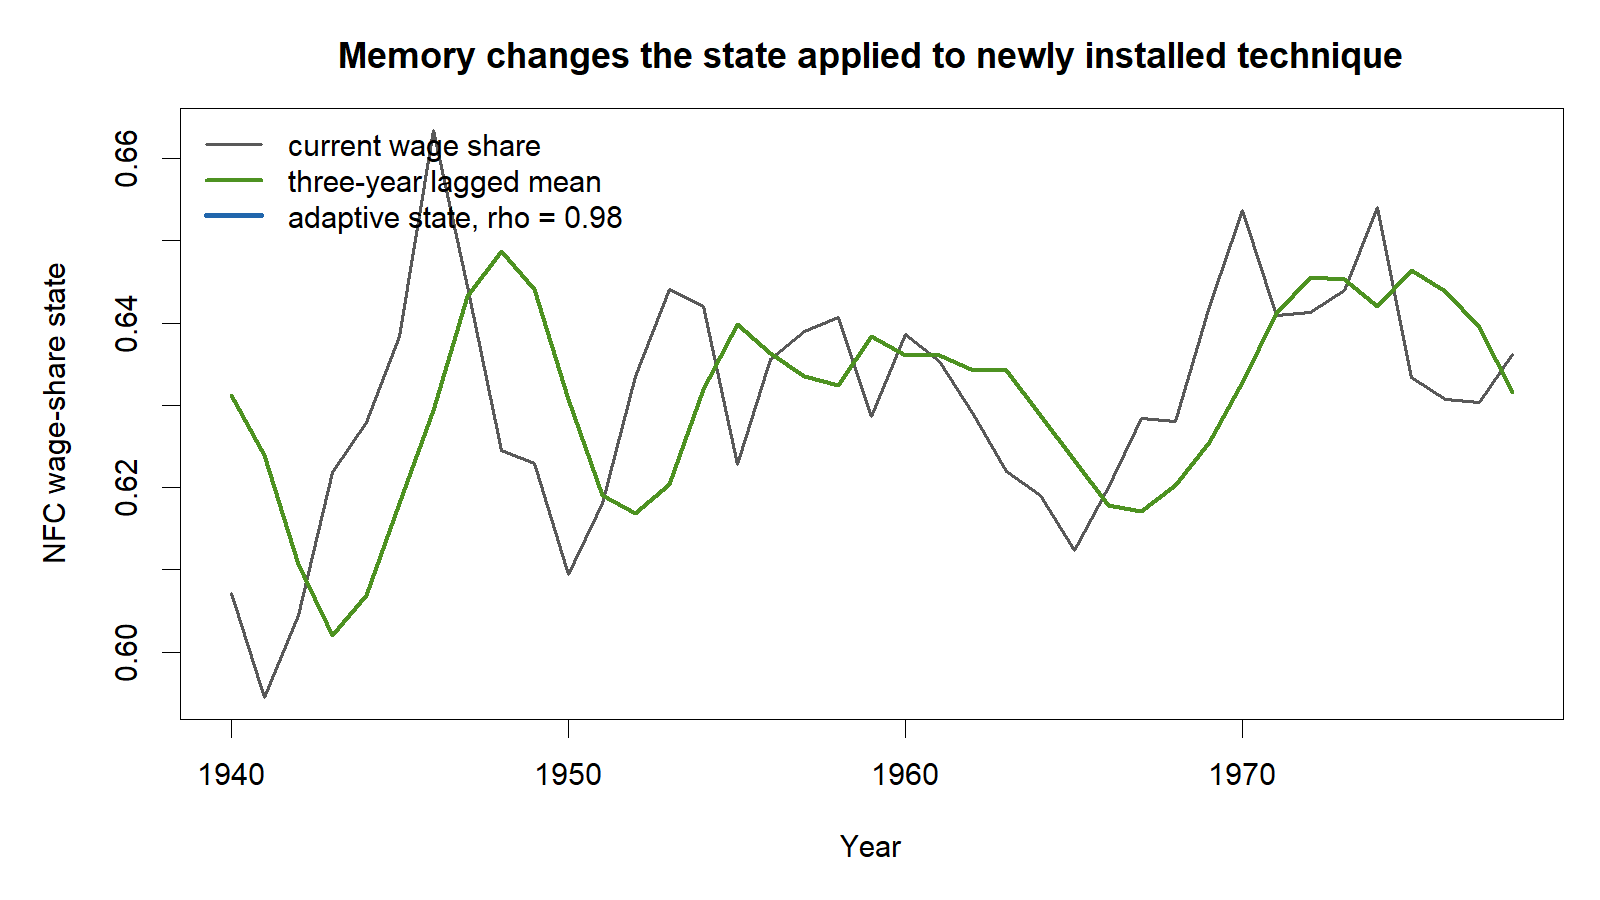
\includegraphics[width=0.95\linewidth]{F11_wage_memory_states.png}
    \end{column}
    \begin{column}{0.39\textwidth}
      \footnotesize
      \begin{description}
        \item[Current state] applies today’s wage share to the entire technique stock.
        \item[Finite memory] replaces today’s share with a lagged moving average.
        \item[Embodiment] weights each new change in machinery intensity by the wage state prevailing when it is installed.
        \item[Adaptive state] estimates how quickly old wage information decays.
      \end{description}
      \begin{block}{Accounting boundary}
        Output and capital remain NFC. Wage pressure is alternately measured for the whole NFC and all corporations; the latter tests a broader bargaining environment.
      \end{block}
    \end{column}
  \end{columns}
  \sourcefooter{\texttt{US\_S90\_path\_dependent\_theta\_robustness.R}: M0, M1, M2, and M3 state constructors}
\end{frame}

% Main 12
\begin{frame}{Persistence is strong; the technique effect is not stable}
  \begin{columns}[T,onlytextwidth]
    \begin{column}{0.57\textwidth}
      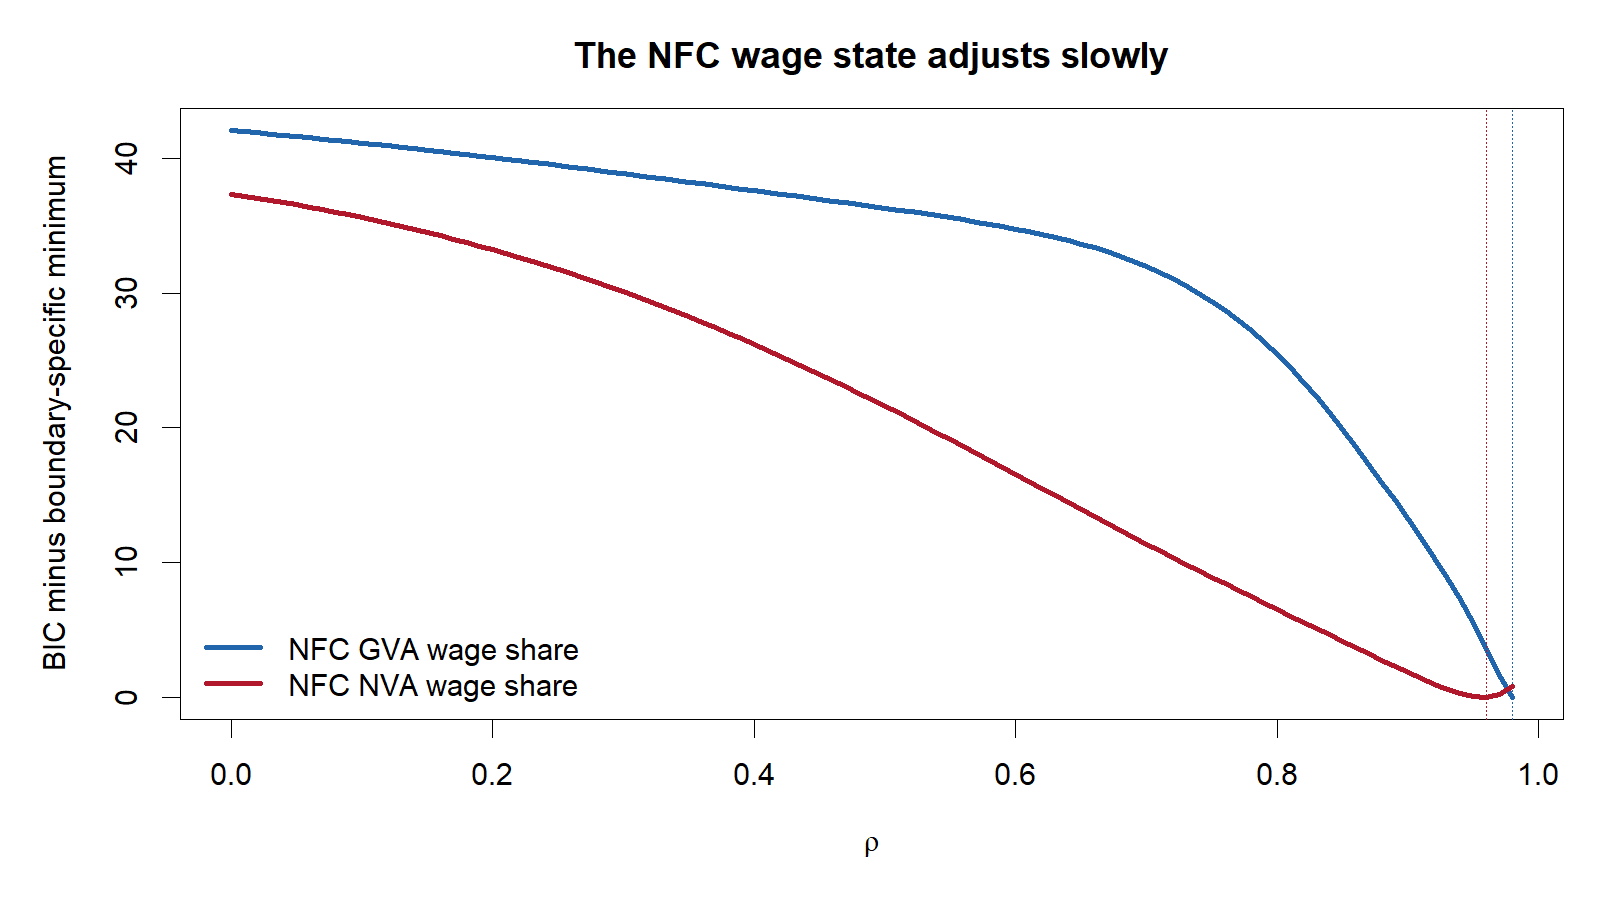
\includegraphics[width=0.92\linewidth]{F10_nfc_persistence_profile.png}
      \vspace{-0.4em}
      \scriptsize
      \begin{tabular}{@{}lccc@{}}
        \toprule
        \textbf{wage state} & $\hat\rho$ & \textbf{block interval} & \textbf{half-life} \\
        \midrule
        NFC GVA & \RhoNfcGva & \RhoNfcGvaLow-\RhoNfcGvaHigh & $\geq\HalfLifeNfcGva$ years \\
        NFC NVA & \RhoNfcNva & \RhoNfcNvaLow-\RhoNfcNvaHigh & \HalfLifeNfcNva\ years \\
        \bottomrule
      \end{tabular}
    \end{column}
    \begin{column}{0.40\textwidth}
      \footnotesize
      \begin{block}{What survives}
        Embodied-memory M2 retains a negative Fordist conditioning effect under both memory lengths:
        \[
        \begin{array}{ll}
        \text{GVA:} & \MtwoLambdaGvaHthree,\ \MtwoLambdaGvaHfive \\
        \text{NVA:} & \MtwoLambdaNvaHthree,\ \MtwoLambdaNvaHfive.
        \end{array}
        \]
      \end{block}
      \begin{alertblock}{Why the full claim fails}
        The GVA persistence estimate reaches the search boundary. M3’s conditioning coefficient also changes sign across GVA (\MthreeLambdaGva) and NVA (\MthreeLambdaNva). Slow memory is evident; a stable equilibrium technique effect is not.
      \end{alertblock}
      \textbf{For v6:} rename the red line, show $g_t^p$ before division, and present memory as qualified evidence.
    \end{column}
  \end{columns}
  \sourcefooter{\texttt{S90\_M3\_persistence\_profile\_ledger.csv} and \texttt{S90\_RDOLS\_coefficient\_ledger.csv}}
\end{frame}

\appendix

% Appendix 1
\begin{frame}{A1. Every displayed result traces to a producing script and artifact}
  \scriptsize
  \renewcommand{\arraystretch}{1.25}
  \setlength{\tabcolsep}{3pt}
  \begin{tabular}{@{}p{0.16\textwidth}p{0.27\textwidth}p{0.245\textwidth}p{0.13\textwidth}p{0.08\textwidth}@{}}
    \toprule
    \textbf{stage} & \textbf{producing script} & \textbf{audited artifact} & \textbf{MD5 prefix} & \textbf{status} \\
    \midrule
    S34 construction & \path{run_s34r_b_cpr_realigned_design_gate.py} & repaired augmented panel & \HashSthirtyFour & PASS \\
    S35 estimation & \path{US_S35_estimator_refreeze_cpr.R} & CPR estimation results & \HashSthirtyFive & PASS \\
    reconstruction & \path{reconstruct_golden_age_paths.R} & Golden-Age reconstructed paths & \HashReconstruction & PASS \\
    S90 diagnostic & \path{US_S90_path_dependent_theta_robustness.R} & S90 coefficient, path, roughness, and persistence ledgers & \HashSninety & PASS \\
    \bottomrule
  \end{tabular}

  \vspace{1em}
  \begin{block}{Audit contract}
    \ClaimCheckCount\ source-to-result claims were independently recomputed. Each row records the script expression, dynamically located source line, input and output artifacts, recomputed value, published value, tolerance, and pass/fail status.
  \end{block}
  \sourcefooter{\texttt{S90\_beamer\_script\_provenance\_ledger.csv} and \texttt{S90\_beamer\_claim\_reproduction\_ledger.csv}}
\end{frame}

% Appendix 2
\begin{frame}{A2. The coefficient-basis audit begins with the actual S34 and S35 code}
  \begin{columns}[T,onlytextwidth]
    \begin{column}{0.50\textwidth}
      \textbf{S34 constructs the full-panel residualized interaction}
      \lstinputlisting{generated/S90_excerpt_S34.txt}
    \end{column}
    \begin{column}{0.48\textwidth}
      \textbf{S35 sends that interaction to the FM-OLS estimator}
      \lstinputlisting{generated/S90_excerpt_S35.txt}
    \end{column}
  \end{columns}
  \vspace{-0.2em}
  \begin{block}{Primitive recovery}
    \centering\small
    $a^{raw}=a^{orth}-\lambda\delta_0$, \quad
    $\theta^{raw}=\theta^{orth}-\lambda\delta_k$, \quad
    $\psi^{raw}=\psi^{orth}-\lambda\delta_{\tau}$, \quad
    $\phi^{raw}=\phi^{orth}-\lambda\delta_d$.
  \end{block}
  \scriptsize Independent residualization agrees with S34 to \texttt{\SthirtyFourResidualDifference}; primitive and orthogonalized fitted values agree to \texttt{\OrthPrimitiveFitDifference}.
  \sourcefooter{Source lines \LineSthirtyFourOrth\ and \LineSthirtyFiveFmols; coefficient values reproduced by \texttt{US\_S90\_beamer\_source\_audit.R}}
\end{frame}

% Appendix 3
\begin{frame}{A3. The two reconstruction boundaries are explicit script facts}
  \begin{columns}[T,onlytextwidth]
    \begin{column}{0.50\textwidth}
      \textbf{Original reconstruction}
      \lstinputlisting[basicstyle=\ttfamily\fontsize{5.0}{5.6}\selectfont]{generated/S90_excerpt_reconstruction.txt}
    \end{column}
    \begin{column}{0.48\textwidth}
      \textbf{S90 reconstruction}
      \lstinputlisting[basicstyle=\ttfamily\fontsize{5.0}{5.6}\selectfont]{generated/S90_excerpt_S90.txt}
    \end{column}
  \end{columns}
  \vspace{-0.55em}
  \begin{columns}[T,onlytextwidth]
    \begin{column}{0.49\textwidth}
      \scriptsize\textbf{Original script:} anchors productive capacity to total real GDP in \AnchorYear, while estimating elasticities from NFC variables.
    \end{column}
    \begin{column}{0.49\textwidth}
      \scriptsize\textbf{S90 script:} fixes observed output at real NFC GVA and anchors every reconstructed $\mu_{\AnchorYear}$ to one.
    \end{column}
  \end{columns}
  \sourcefooter{Boundary claims \texttt{SRC\_RECON\_OUTPUT\_BOUNDARY} and \texttt{SRC\_S90\_OUTPUT\_BOUNDARY} in the claim ledger}
\end{frame}

% Appendix 4
\begin{frame}{A4. Reproduction succeeds before the expanded deck is compiled}
  \begin{columns}[T,onlytextwidth]
    \begin{column}{0.50\textwidth}
      \begin{block}{Execution}
        \small
        \texttt{Rscript}\hspace{0.35em}\path{codes/US_S90_beamer_source_audit.R}

        \vspace{0.5em}
        Required estimator package: \texttt{cointReg}.
      \end{block}
      \begin{block}{Numerical checks}
        \small
        \begin{itemize}
          \item \ClaimCheckCount\ source-to-result claims: all PASS
          \item \ValidationCheckCount\ S90 identities: all PASS
          \item \BootstrapReplications\ moving-block draws per wage boundary
          \item coefficient tolerance: $\CoefficientTolerance$
          \item algebraic identities: $\AlgebraTolerance$ or tighter
        \end{itemize}
      \end{block}
    \end{column}
    \begin{column}{0.47\textwidth}
      \begin{block}{Generated interfaces}
        \small
        \begin{itemize}
          \item script provenance ledger
          \item source-anchor ledger
          \item claim-reproduction ledger
          \item generated TeX number macros
          \item verbatim code excerpts
        \end{itemize}
      \end{block}
      \begin{alertblock}{Preservation boundary}
        The audit writes only new S90 presentation assets. The v6 PDF, the six-slide addendum, S40, and Stage B/C remain unchanged.
      \end{alertblock}
    \end{column}
  \end{columns}
  \sourcefooter{\texttt{S90\_BEAMER\_SOURCE\_AUDIT.md} and \texttt{S90\_validation\_checks.csv}}
\end{frame}

\end{document}
